\documentclass{../letter}
\usepackage{cite}

\newcommand{\E}{$\mathbb{E}^3$}
\newcommand{\eq}[1]{Eq.~\eqref{#1}}
\newcommand{\eqs}[1]{Eqs.~\eqref{#1}}
\newcommand{\fig}[2][\empty]{Figure \hyperref[fig:#2]{\ref{fig:#2}#1}}

\begin{document}
	\header{Caltech SURF Project Proposal}

	\section{Introduction \& Background}

	In most introductory General Relativity textbooks, authors embed 2-dimensional geometries in flat 3-dimensional space (\E) \cite[chapter 2]{hartle}. This is the idea for the ``isometric embedding problem'', which we can use to find the shape that a black hole apparent horizon \textit{would have} if it lived in \E. In order to accomplish such task, one needs to solve a system of 3 nonlinear partial differential equations,
	\begin{equation}\label{embedding}
		\begin{cases}
			(\partial_\theta x)^2 + (\partial_\theta y)^2 + (\partial_\theta z)^2 = g_{\theta\theta} \\
			(\partial_\phi x)^2 + (\partial_\phi y)^2 + (\partial_\phi z)^2 = g_{\phi\phi} \\
			(\partial_\theta x) (\partial_\phi x) + (\partial_\theta y) (\partial_\phi y) + (\partial_\theta z) (\partial_\phi z) = g_{\theta\phi}
		\end{cases},
	\end{equation}
	where $\{\theta, \phi\}$ are angle coordinates, $\{x(\theta,\phi), y(\theta,\phi), z(\theta,\phi)\}$ are the embedding functions we want to find and $(g_{\alpha\beta})$ is the metric describing the surface.

	Professor Robert Owen has been investigating the embedding problem for over 5 years, working with many students at Oberlin College. I started working with Professor Owen during my first in-person semester at Oberlin in the Fall of 2021. Now, I am in my third year working on this research, which turned into my Honors thesis. Our main goal has been to develop an efficient algorithm capable of solving \eqs{embedding}. As a result of my research efforts, I became a member of the SXS collaboration and presented at the APS April 2023 Meeting \cite{APS_poster}.

	We have successfully developed two algorithms in SpEC \cite{SpEC} that approach the embedding problem in significantly different ways and accomplish similar results. When using our methods in binary black hole merger simulations, we found special scenarios in which the embeddings are a better representation of the physics occurring in the horizon compared to the standard coordinate shape. Examples are shown in \fig{comparison}. We plan to publish a paper sharing our results in the near future.

	% \twoImages
	% 	{assets/AntiAligned_PreMerger.png}{fig:PreMerger}
	% 	{assets/NonSpinning_CommonHorizon.png}{fig:CommonHorizon}
	% 	{Extreme comparisons between coordinate shapes and isometric embeddings taken from an antialigned inspiral simulation. (a) Shows the binary black holes pre-merger. (b) Shows the recently formed common horizon.}
	
	\begin{figure}[H]
		\centering
		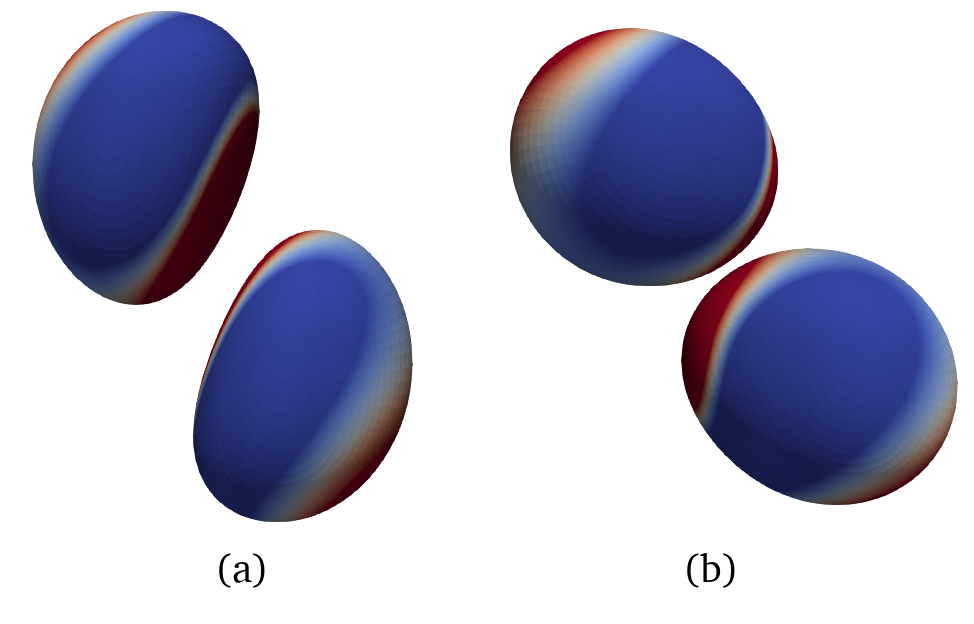
\includegraphics[height=120px]{assets/NonSpinning_PreMerger.png}
		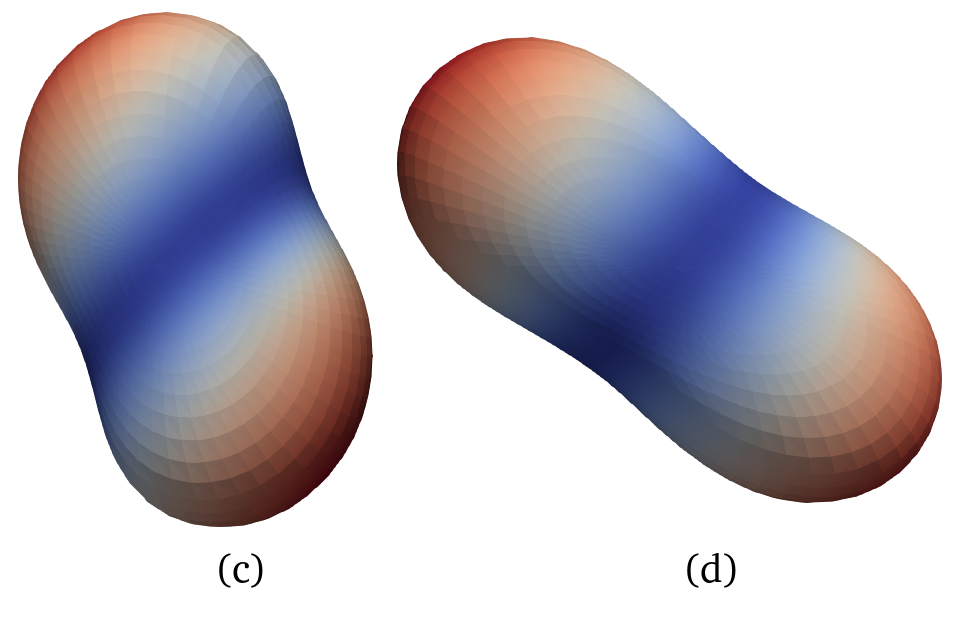
\includegraphics[height=120px]{assets/NonSpinning_PostMerger.png}
		\caption{Comparison between coordinate shapes (a, c) and isometric embeddings (b, d) of apparent horizons for a simulation of equal-mass non-spinning black holes, just before and just after merger. Red and blue indicate high and low curvature, respectively.}
		\label{fig:comparison}
	\end{figure}

	In this document, I propose a research project to be conducted with Caltech researchers that are members of the SXS collaboration as part of the SURF program. As I explain in the next section, my proposal is to expand on my previous work on the embedding problem.

	\section{Objectives}

	First, it is important to note that I am open to work on any project that might be of interest to the SXS collaboration. Having prior experience with SpEC development and industry software engineering, I am confident that I would be able to make significant contributions to Numerical Relativity projects that the research group might currently have for SpEC or SpECTRE. That said, I list below some interesting research projects that would follow up on my research of the embedding problem.

	\subsection{Critical embedding}

	It is known that not all curved surfaces can be embedded using \eqs{embedding}. Perhaps the most famous example is when a Kerr black hole has a dimensionless spin $a/M \gtrsim 0.86$ \cite[chapter 15]{hartle}. Be as it may, it is not currently well understood how horizons in generic simulations transition from an embeddable surface to a non-embeddable one. We have found examples of non-embeddable surfaces in our code that are far more generic than the Kerr horizon. In \fig{nonembeddable}, we can clearly see non-physical features near the poles of the embedding for the recently-formed common horizon, which we believe to indicate non-embeddability. This belief is based on the fact that these features are seen in the results from both embedding methods around the same evolution time.

	\begin{figure}[H]
		\centering
		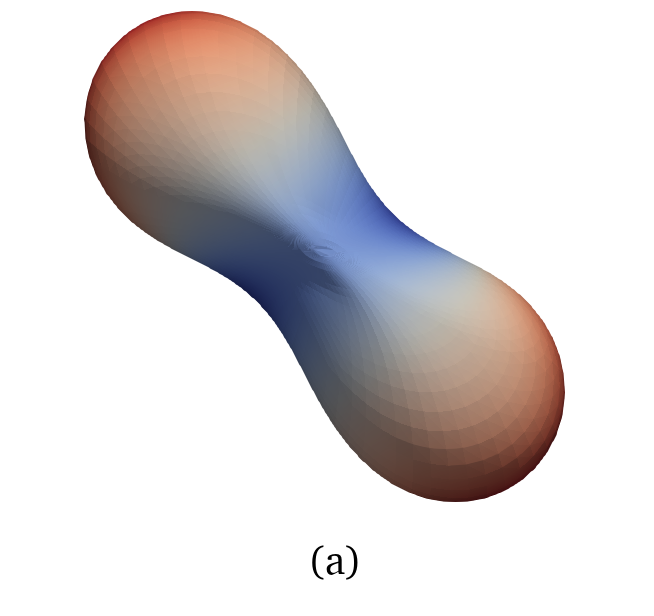
\includegraphics[height=120px]{assets/AntiAlignedSharp_Relaxation.png}
		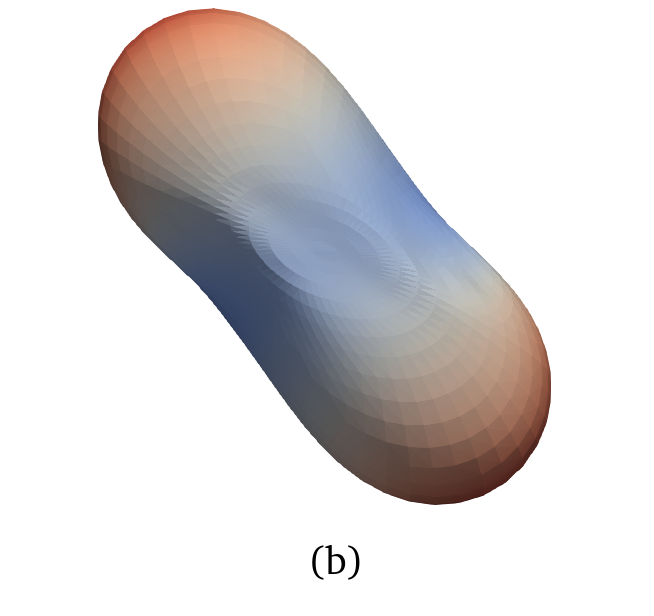
\includegraphics[height=120px]{assets/AntiAlignedSharp_Matrix.png}
		\caption{Examples of non-physical features in isometric embeddings of the common apparent horizon for a simulation of equal-mass antialigned black holes, just after merger. (a) and (b) show results from our relaxation and matrix methods, respectively.}
		\label{fig:nonembeddable}
	\end{figure}
	
	The study of this ``critical embedding'' would considerably benefit from our previous work on the embedding problem. In this project, we would run several black hole simulations, analyzing which conditions could be associated with the embeddability of the apparent horizon and how this transition occurs. Our hypothesis is that the breakdown of embeddability behaves in an analogous way to different processes that are currently understood. Possible analogies include the relativistic collapse during black hole formation (in which the energy density is the determining factor) and phase transitions in Statistical Mechanics.

	\subsection{Inspecting gauge conditions}

	In numerical relativity, spatial coordinates evolve over time via a gauge condition. In SpEC, this condition is chosen to provide good numerical stability, but does not guarantee a minimization of unphysical distortions. \fig[a]{comparison} shows that these distortions can occur especially near merger, when the simulation runs slower due to a need for higher resolution.
	
	A reasonable hypothesis is that the merger phase would run more efficiently if the spatial coordinates were less distorted. The argument is that, with fewer distortions, we could lower the resolution in order to speed up the merger phase. To accomplish this, we would need to choose gauge conditions that minimize such distortions, which would only be possible if we have a way to measure distorted coordinates.
	
	Now that we have developed a method for finding horizon embeddings, we have a possible representation of distortions. That is, the difference between the isometric embedding and the coordinate shape for a given horizon could potentially be used as a distortion measure. From \fig[a]{comparison} and \fig[b]{comparison}, it is clear that there are cases in which the intrinsic geometry is more round than the coordinate shape indicates, possibly suggesting that the gauge conditions could be optimized.
	
	In summary, this project would attempt to use isometric embeddings to measure unphysical distortions, which would then be used as a determining factor for choosing gauge conditions. If successful, this would optimize the merger phase of binary black hole simulations.

	\subsection{Wang-Yau quasilocal mass}

	In 2009, Mu-Tao Wang and Shing-Tung Yau proposed a new notion of the quasilocal mass for horizons \cite{WangYau_2009}. This definition relies on embedding the apparent horizon into Minkowski space. In 2023, Yau and collaborators studied this quasilocal mass on head-on simulations of binary non-spinning black holes \cite{Yau_2023}. Due to limitations on their embedding method, they were not able to study more complex simulations.

	With the embedding methods that we have developed, SpEC is now capable of finding the isometric embedding for many generic horizons. The way it is currently implemented, we are only able to embed horizons into Euclidean space, but it should be possible to expand our approach to include the time embedding function so that we can embed horizons into Minkowski space.

	It is important to note that this is the immediate goal for our research group at Oberlin, especially because we have already met with Yau and collaborators, who showed interest in our method. Given the time separation between the submission of this document and the start of the program, it is possible that we finish adapting our methods to the Wang-Yau quantity before the summer. In such case, a possible follow-up project would be to analyze the properties of the quasilocal mass in generic simulations, expanding on the results recently shared by Yau and collaborators in \cite{Yau_2023}.

	\section{Approach}

	\section{Work Plan}

	\bibliographystyle{plain}
	\bibliography{refs}
\end{document}
